\documentclass[leqno, openany]{memoir}
\setulmarginsandblock{3.5cm}{3.5cm}{*}
\setlrmarginsandblock{3cm}{3.5cm}{*}
\checkandfixthelayout

\usepackage{amsmath}
\usepackage{amssymb}
\usepackage{amsthm}
%\usepackage{MnSymbol}
\usepackage{bm}
\usepackage{accents}
\usepackage{mathtools}
\usepackage{tikz}
\usetikzlibrary{calc}
\usetikzlibrary{automata,positioning}
\usepackage{tikz-cd}
\usepackage{forest}
\usepackage{braket} 
\usepackage{listings}
\usepackage{mdframed}
\usepackage{verbatim}
\usepackage{physics}
%\usepackage{/home/patrickl/homework/macaulay2}

%font
\usepackage[osf]{mathpazo}
\usepackage{microtype}

%CS packages
\usepackage{algorithmicx}
\usepackage{algpseudocode}
\usepackage{algorithm}

% typeset and bib
\usepackage[english]{babel} 
\usepackage[utf8]{inputenc} 
\usepackage[backend=biber, style=alphabetic]{biblatex}
\usepackage[bookmarks, colorlinks, breaklinks]{hyperref} 
\hypersetup{linkcolor=black,citecolor=black,filecolor=black,urlcolor=black}

% other formatting packages
\usepackage{float}
\usepackage{booktabs}
\usepackage{enumitem}
\usepackage{csquotes}
\usepackage{titlesec}
\usepackage{titling}
\usepackage{fancyhdr}
\usepackage{lastpage}
\usepackage{parskip}

\usepackage{lipsum}

% delimiters
\DeclarePairedDelimiter{\gen}{\langle}{\rangle}
\DeclarePairedDelimiter{\floor}{\lfloor}{\rfloor}
\DeclarePairedDelimiter{\ceil}{\lceil}{\rceil}


\newtheorem{thm}{Theorem}[section]
\newtheorem{cor}[thm]{Corollary}
\newtheorem{prop}[thm]{Proposition}
\newtheorem{lem}[thm]{Lemma}
\newtheorem{conj}[thm]{Conjecture}
\newtheorem{quest}[thm]{Question}

\theoremstyle{definition}
\newtheorem{defn}[thm]{Definition}
\newtheorem{defns}[thm]{Definitions}
\newtheorem{con}[thm]{Construction}
\newtheorem{exm}[thm]{Example}
\newtheorem{exms}[thm]{Examples}
\newtheorem{notn}[thm]{Notation}
\newtheorem{notns}[thm]{Notations}
\newtheorem{addm}[thm]{Addendum}
\newtheorem{exer}[thm]{Exercise}

\theoremstyle{remark}
\newtheorem{rmk}[thm]{Remark}
\newtheorem{rmks}[thm]{Remarks}
\newtheorem{warn}[thm]{Warning}
\newtheorem{sch}[thm]{Scholium}


% unnumbered theorems
\theoremstyle{plain}
\newtheorem*{thm*}{Theorem}
\newtheorem*{prop*}{Proposition}
\newtheorem*{lem*}{Lemma}
\newtheorem*{cor*}{Corollary}
\newtheorem*{conj*}{Conjecture}

% unnumbered definitions
\theoremstyle{definition}
\newtheorem*{defn*}{Definition}
\newtheorem*{exer*}{Exercise}
\newtheorem*{defns*}{Definitions}
\newtheorem*{con*}{Construction}
\newtheorem*{exm*}{Example}
\newtheorem*{exms*}{Examples}
\newtheorem*{notn*}{Notation}
\newtheorem*{notns*}{Notations}
\newtheorem*{addm*}{Addendum}


\theoremstyle{remark}
\newtheorem*{rmk*}{Remark}

% shortcuts
\newcommand{\Ima}{\mathrm{Im}}
\newcommand{\A}{\mathbb{A}}
\newcommand{\N}{\mathbb{N}}
\newcommand{\R}{\mathbb{R}}
\newcommand{\C}{\mathbb{C}}
\newcommand{\Z}{\mathbb{Z}}
\newcommand{\Q}{\mathbb{Q}}
\renewcommand{\k}{\Bbbk}
\renewcommand{\P}{\mathbb{P}}
\newcommand{\M}{\overline{M}}
\newcommand{\g}{\mathfrak{g}}
\newcommand{\h}{\mathfrak{h}}
\newcommand{\n}{\mathfrak{n}}
\renewcommand{\b}{\mathfrak{b}}
\newcommand{\ep}{\varepsilon}
\newcommand*{\dt}[1]{%
   \accentset{\mbox{\Huge\bfseries .}}{#1}}
\renewcommand{\abstractname}{Official Description}
\newcommand{\mc}[1]{\mathcal{#1}}
\newcommand{\T}{\mathbb{T}}
\newcommand{\mf}[1]{\mathfrak{#1}}
\newcommand{\mr}[1]{\mathrm{#1}}
\newcommand{\ms}[1]{\mathsf{#1}}
\newcommand{\ol}[1]{\overline{#1}}
\newcommand{\wt}[1]{\widetilde{#1}}

\DeclareMathOperator{\Der}{Der}
\DeclareMathOperator{\Hom}{Hom}
\DeclareMathOperator{\colim}{colim}
\DeclareMathOperator{\End}{End}
\DeclareMathOperator{\ad}{ad}
\DeclareMathOperator{\Aut}{Aut}
\DeclareMathOperator{\Rad}{Rad}
\DeclareMathOperator{\supp}{supp}
\DeclareMathOperator{\sgn}{sgn}
\DeclareMathOperator{\spec}{Spec}

% Section formatting
\titleformat{\section}
    {\Large\sffamily\scshape\bfseries}{\thesection}{1em}{}
\titleformat{\subsection}[runin]
    {\large\sffamily\bfseries}{\thesubsection}{1em}{}
\titleformat{\subsubsection}[runin]{\normalfont\itshape}{\thesubsubsection}{1em}{}

\title{COURSE TITLE}
\author{Lectures by INSTRUCTOR, Notes by NOTETAKER}
\date{SEMESTER}

\newcommand*{\titleSW}
    {\begingroup% Story of Writing
    \raggedleft
    \vspace*{\baselineskip}
    {\Huge\itshape Algebraic Topology \\ Fall 2020}\\[\baselineskip]
    {\large\itshape Notes by Patrick Lei}\\[0.2\textheight]
    {\Large Lectures by Mohammed Abouzaid}\par
    \vfill
    {\Large \sffamily Columbia University}
    \vspace*{\baselineskip}
\endgroup}
\pagestyle{simple}

\chapterstyle{ell}


%\renewcommand{\cftchapterpagefont}{}
\renewcommand\cftchapterfont{\sffamily}
\renewcommand\cftsectionfont{\scshape}
\renewcommand*{\cftchapterleader}{}
\renewcommand*{\cftsectionleader}{}
\renewcommand*{\cftsubsectionleader}{}
\renewcommand*{\cftchapterformatpnum}[1]{~\textbullet~#1}
\renewcommand*{\cftsectionformatpnum}[1]{~\textbullet~#1}
\renewcommand*{\cftsubsectionformatpnum}[1]{~\textbullet~#1}
\renewcommand{\cftchapterafterpnum}{\cftparfillskip}
\renewcommand{\cftsectionafterpnum}{\cftparfillskip}
\renewcommand{\cftsubsectionafterpnum}{\cftparfillskip}
\setrmarg{3.55em plus 1fil}
\setsecnumdepth{subsection}
\maxsecnumdepth{subsection}
\settocdepth{subsection}

\begin{document}
    
\begin{titlingpage}
\titleSW
\end{titlingpage}

\thispagestyle{empty}
\section*{Disclaimer}%
\label{sec:disclaimer}

These notes were taken during lecture using the \texttt{vimtex} package of the editor \texttt{neovim}. 
Any errors are mine and not the instructor's. 
In addition, my notes are picture-free (but will include commutative diagrams) and are a mix of my mathematical style and that of the instructor.
If you find any errors, please contact me at \texttt{plei@math.columbia.edu}.
\newpage


\tableofcontents

\chapter{Basics of Homotopy Theory}%
\label{cha:basic_notions}

\section{Categorical Notions}%
\label{sec:categorical_notions}

We will use the book \textit{Algebraic Topology} by Tammo tom Dieck. We will use categorical language, even if we don't strictly need it. We will denote the category of (Hausdorff) topological spaces and continuous maps by $\ms{Top}$. There are two ways of thinking about algebraic topology:
\begin{enumerate}
    \item Extracting algebraic invariants from spaces;
    \item Doing algebra with spaces.
\end{enumerate}

Homotopy is an equivalence relation on $\ms{Top}(X,Y)$. 

\begin{defn}
    A \textit{homotopy} from $f$ to $g$ is a map $H: X \times I \to Y$ such that $H \circ i_0 = f$ and $H \circ i_1 = g$. Intuitively, this is a way to interpolate between $f$ and $g$. Alternatively, a homotopy is a path in $Y^X$ with the compact-open topology.
\end{defn} 

To show that homotopy is an equivalence relation, it is easy to show that $f$ is self-homotopic. To see that homotopy is symmetric, we can simply reverse the interval. Finally, to see that homotopy is transitive, we can just perform each homotopy twice as fast and then concatenate.

\begin{defn}
The \textit{homotopy category} $\ms{hTop}$ is the category whose objects are spaces and whose morphisms are homotopy classes of maps. We need to check that composition preserves the notion of homotopy.
\end{defn}

Now denote the \textit{category of based spaces} by $\ms{Top}^*$, where a based space is a space $X$ with a map $* \to X$. The corresponding homotopy category is denoted by $\ms{hTop}^*$. Here, the homotopy is required to fix the basepoint.

\begin{rmk}
    The transition from spaces to based spaces is like upgrading from semigroups to monoids.
\end{rmk}

\begin{rmk}
    There is a functor 
    \begin{align*}
        \ms{Top} \to \ms{Top}^* \\
        X \mapsto (X \sqcup \{*\}, *).
    \end{align*}
\end{rmk}

\begin{exm}
    It is easy to see that $\ms{Top}(*,X) \cong X$. Similarly, $\ms{Top}^*(S^0,(X,*)) \cong X$. Then, we can see that $\ms{hTop}(*,X) \cong \ms{hTop}(S^0,X)$ is the set of path components of $X$.
\end{exm}

\section{Fundamental Group and Groupoid}%
\label{sec:fundamental_group_and_groupoid}

\begin{exm}
    We will now consider morphisms from the circle. The set $\ms{Top}(S^1,X)$ is the free loop space $\mc{L}X$. In the based case, we get the \textit{based loop space} $\Omega X$. Then $\ms{hTop}(S^1,X)$ is the path components of $\mc{L}X$, and similarly, $hTop^*(S^1,X) \cong \pi_1(X,*)$, where $\pi_1$ is the fundamental group.
\end{exm}

It should be surprising that $[S^1,X]$ is a group. In fact, it is independent on the path component of $*$ up to inner automorphism. However, we can distinguish a class of isomorphisms up to conjugation. The identity of this group is the constant path at the basepoint. Next, we need to consider the product in the group. This is simply concatenation, which is given by the (cogroup) operation $S^1 \to S^1 \vee S^1$. Because the two components of the wedge cannot be swapped by a homotopy, this operation is not commutative.

Next, we need to check that this is compatible with homotopy. Then the operation on homotopy classes is the product in $\pi_1$. To check associativity, we can check that the total operation of pinching at $1/3$ and pinching at $2/3$ commutes.

Finally, the inverse of a path $g$ is simply $t \mapsto g(1-t)$. To construct an isomorphism between $\pi_1(X,*_1)$ and $\pi_1(X, *_2)$, choose a path $g$ between the two basepoints and then send $f \mapsto g^{-1} f g$.

We will now discuss an unbased analogue of the fundamental group. Beginning with the path space $\mathsf{Top}([0,1],X)$, we can consider the evaluations at $0$ and $1$. Then over $(x,y)$, can consider homotopy classes of maps with fixed endpoints to obtain the set $\Pi X(x,y)$.

\begin{prop}
    $\Pi X(x,y)$ are the morphisms of a \textit{groupoid} with objects $X$.
\end{prop}

\begin{rmk}
    $\Pi X(x,x) \cong \pi_1(X,x)$. The fundamental group is much nicer, but is hard to compute because it depends on the basepoint.
\end{rmk}

\begin{defn}
    A \textit{homotopy equivalence} $f:X \to Y$ is a map that induces an isomorphism in the homotopy category. 
\end{defn}

\begin{prop}
    A homotopy equivalence $X \to Y$ induces an equivalence of categories $\Pi f: \Pi X \to \Pi Y$. Recall here that an equivalence of categories is a fully faithful and essentially surjective functor. Equivalently, it is a functor has an inverse up to natural isomorphism.
\end{prop}

\begin{proof}
    The homotopy defines a natural transformation from $\mr{id}_X$ to $\Pi gf$. Let $g$ be a homotopy inverse, and $H$ be a homotopy and let $H$ be a homotopy from $\mr{id}_X$ to $gf$. We can evaluate $H$ on the path $\gamma$, and this gives a homotopy between $x \to y \to g(f(y))$ and $x \to g(f(x)) \to g(f(y))$. Therefore, we have equality up to homotopy, so this gives a natural transformation. Because we are working in a groupoid, this is automatically an isomorphism.
\end{proof}

\begin{cor}
    Homotopy equivalences induce isomorphisms of fundamental groups.
\end{cor}

Suppose we have a diagram of the form
\begin{equation}
\begin{tikzcd}
    A \arrow{r}{f_1} \arrow{d}{f_2} & B_1 \\
    B_2
\end{tikzcd}.
\end{equation}
Then a \textit{pushout} $C$ is the colimit of this diagram. This means that there exist maps $g_1, g_2$ such that
\begin{equation}
\begin{tikzcd}
    A \arrow{r}{f_1} \arrow{d}{f_2} & B_1 \arrow{d}{g_1} \\
    B_2 \arrow{r}{g_2} & C
\end{tikzcd}
\end{equation}
commutes and $(C, g_1, g_2)$ is universal: For any $X$ and commutative diagram, there exists a unique map such that
\begin{equation}
\begin{tikzcd}
    A \arrow{r}{f_1} \arrow{d}{f_2} & B_1 \arrow{d}{g_1} \arrow{ddr} & \\
    B_2 \arrow{r}{g_2} \arrow{drr} & C \arrow[dashrightarrow]{dr} &  \\
                                   & & X
\end{tikzcd}
\end{equation}
commutes.

\begin{thm}[Seifert-van Kampen Theorem]
    Let $X$ be a topological space and $X_0, X_1$ subspaes whose interiors cover $X$. Then set $X_{01} = X_0 \cap X_1$. Then 
\begin{equation}
\begin{tikzcd}
    \Pi X_{01} \arrow{r} \arrow{d} & \Pi X_0 \arrow{d} \\
    \Pi X_1 \arrow{r} & \Pi X
\end{tikzcd}
\end{equation}
is a pushout diagram of groupoids.
\end{thm}

\begin{proof}
    Consider a groupoid $G$ and commutative diagram
\begin{equation}
\begin{tikzcd}
    \Pi X_{01} \arrow{r}{f_0} \arrow{d}{f_1} & \Pi X_0 \arrow{d}{h_0} \\
    \Pi X_1 \arrow{r}{h_1} & G
\end{tikzcd}.
\end{equation}
We will construct $\Pi X \xrightarrow{h} G$. Then we need to write $h(x)$ as an object of $G$. If $x \in X_1$, set $h(x) = h_1(x)$, and if $x \in X_0$, set $h(x) = h_0(x)$. Because (1.5) commutes, this is well-defined. Now we define $h$ on the level of morphisms. Subdivide paths so that all segments lie in either $X_0$ or $X_1$. Then on each such segment, the diagram specifies $h(\gamma_i)$, and define $h(\gamma) = h(\gamma_0) h(\gamma_1) \cdots h(\gamma_n)$.

Finally, we need to prove that this definition is independent of the choice of representative of homotopy class. We can subdivide the homotopy so each equare lies in either $X_0$ or $X_1$, and then $h_1, h_1$ are well-defined, so $h$ is independent of the homotopy class.
\end{proof}

\begin{exm}
    We can use Seifert-van Kampen to compute the fundamental group of $S^1$. If we choose $X_0. X_1$ to be two arcs, then $X_{01}$ is homotopy equivalent to two points. Then computing combinatorially, we can recover $\pi_1(S^1, *) \cong \Z$.
\end{exm}

\begin{cor}[Standard statement of Seivert-van Kampen]
    For connected $X_{01}$, we obtain a pushout diagram in the category of \textit{groups}. 
\end{cor}

\section{Covering Spaces}%
\label{sec:covering_spaces}

\begin{defn}
Let $B$ be a topological space. Then $p:E \to B$ is a \textit{covering map} if it is locally trivial with discrete fiber. 
\end{defn}

\begin{exm}
    Consider $S^1 \times \Z \to S^1$. Another covering map to $S^1$ with fiber $\Z$ is the projection $\R \to \R / \Z = S^1$.
\end{exm}

\begin{prop}
    Every covering of $I$ is trivial.
\end{prop}

\begin{proof}
    Let $F = p^{-1}(0)$. Then over $U_x \ni x$, we can trivialize the cover. Because $I$ is compact, we can choose a finite cover $\{ U_i\}$ over which $p$ is trivial. By indexing the $U_i$ and removing the unnecessary ones, we can assume $U_i \cap U_j \neq \emptyset$ if and only if $i - j = \pm 1$. By induction, we want to extend the trivialization on the first $n$ elements of the cover to the union with $U_{n+1}$. The trivialization gives us an isomorphism $p^{-1}(0) \cong p^{-1}(t)$ for all $t \in U_n$, so if $t \in U_{n+1}$, we the local trivialization to obtain an isomorphism $p^{-1}(t) \cong p^{-1}(t')$ for all $t' \in U_{n+1}$. Then compose $p^{-1}(0) \cong p^{-1}(t) \cong p^{-1}(t')$. The procedure terminates by compactness.
\end{proof}

To generalize this result to contractible spaces, we need more tools. The limit of the diagram
\begin{equation}
\begin{tikzcd}
    & E \arrow{d}{p} \\
    X \arrow{r}{i} & B
\end{tikzcd}
\end{equation}
is called the \textit{pullback}. 

\begin{lem}
    The pullback of a cover is a cover.
\end{lem}

\begin{proof}
    If $E \to B$ is trivial over $U \subset B$, then $i^* E$ is trivial over $f^{-1}(U) \subset X$.
\end{proof}

\begin{lem}
    A homotopy $X \times I \xrightarrow{f} B$ induces an isomorphism of covers
    \begin{equation}
    \begin{tikzcd}
        f_0^* E \arrow{rr}{f_*} \arrow{dr} & & f_1^* E \arrow{dl} \\
                                           & X &
    \end{tikzcd}
    \end{equation}
\end{lem}

\begin{proof}
    Use the idea of the proof in the case of the interval. We can transport the fibers from $f_0$ to $f_1$, so this gives a homeomorphism.
\end{proof}

\begin{cor}
    If $X$ is contractible, all covers are trivial.  
\end{cor}

\begin{proof}
    Then choose $H_0 = \mr{id}$ and $H_1$ to be constant at $x$. Then we obtain a homeomorphism between $E \to X$ and $X \times p^{-1}(x) \to X$.
\end{proof}

\begin{cor}
    If $p: E \to B$ is a cover, then the assignment $b \to E_b = p^{-1(b)}, \gamma \to \gamma_{\alpha}$ defines a functor $T_p: \Pi B \to \ms{Set}$.
\end{cor}

\begin{defn}
    A cover $\wt{B} \xrightarrow{p} B$ is a \textit{universal cover} if there exists $b_0$ to $B$ such that $T_p$ is isomorphic to the functor $b \to \Pi(b,b_0)$ (equivalently if $T_p$ is representable).
\end{defn}

\begin{lem}
    If $B$ is locally simply connected and path connected, then the universal cover exists.
\end{lem}

\begin{proof}
    We will build the space by equipping $\wt{B} = \bigsqcup_b \Pi(b,b_0)$ with a topology. We want locally that $\wt{B}$ is homeomorphic to $U \times \Pi(b,b_0)$. At every point $b \in B$, we can choose $U$ which is path connected and simply connected. In $U$, there is a canonical isomorphism $\Pi(b_0,b) \cong \Pi(b_0,b')$ because between any two points, there is a unique homotopy class of paths between them. This determines the topology.
\end{proof}

Note, $\wt{B} = E$ is a principal $G \coloneqq \pi_1(B,b_0)$ bundle over $B$. In particular, the map $G \times E \to E$ is equivariant over $B$ and $G \times E_b \to E_b$ is isomorphic to $G \times G \to G$.

Now we will give a classification of coverings. Assume the universal cover exists. Then there exists a bijection between the following data:
\begin{enumerate}
    \item Coverings $E \to B$ up to isomorphism.
    \item Functors $\Pi B \to \ms{Set}$ up to isomorphism.
    \item Actions of $\pi_1(B,b_0)$ on a set $F$ up to isomorphism.
\end{enumerate}

\begin{proof}
    The bijection between 1 and 2 is given by the transport functor. Between 2 and 3, we simply restrict the functor to a single object. Finally, we can consider the associated bundle $\wt{B} \times F / \pi_1(B,b_0)$.
\end{proof}

\begin{defn}
    A cover $E \to B$ is \textit{regular} if there exists a norma subgroup of $\pi_1(B,b_0)$ such that $p^{-1}(b_0) \cong \pi_1(B,b_0) / N$.
\end{defn}

This implies that $E$ is a principal $H$-bundle for a quotient $H$ of $\pi_1(B,b_0)$, and in fact this is an equivalence.

How do we recognize the universal cover? Let $E \to B$ be a cover. Fix basepoints $b, \wt{b}$ and consider the map $\pi_1(E, \wt{b}) \to \pi_1(B,b)$. 
\begin{description}
    \item[Homotopy Lifting Property:] Consider two paths $\gamma_0, \gamma_1$ in $B$ with the same endpoints. Then if we consider the diagram
        \begin{equation}
        \begin{tikzcd}
            I \times \{ 0,1 \} \arrow{r} \arrow{d} & \wt{B} \arrow{d}{p} \\
            I \times I \arrow{r}{H} & B,
        \end{tikzcd}
        \end{equation}
        there is a unique $I \times I \to \wt{B}$ such that the entire diagram commutes.

        To prove this, we can consider the pullback $p^*(H)$, which is a cover of $I \times I$, which is trivial. This property implies the map on $\pi_1$ is injective.
    \item[Transport:] The transport of $\wt{b}$ defines a map $\pi_1(B,b) \to \pi_0(E_b, \wt{b})$ and the ``kernel'' agrees with $\pi_1(E, \wt{b})$. The inclusion of $\pi_1(E)$ in the kernel comes from the homotopy lifting property, and in the other direction, any loop that lifts to a path taking $\wt{b}$ to itself must have come from a loop.
    \item[Components of the cover:] If $B$ is path connected, then $\pi_0(E_b,\wt{b}) / \pi_1(B,b) \cong \pi_0(E,\wt{b})$.

        To see this, we will map $\pi_0(E_b, \wt{b}) \to \pi_0(E, \wt{b})$ induced by the inclusion $E_b \subset E$. To check that this is well-defined, note that each $\gamma \in \pi_1(B,b)$ lifts to a path between two points of $E_b$. To check surjectivity, choose $x \in E$ and $p(x)$ the projection. Choose a path $\gamma$ from $p(x)$ to $b$ and then transport from the fiber at $b$ to $x$. To show injectivity, we simply use the homotopy lifting property. If $f, f'$ are points in $E_b$ lying in the same component of $E$, we can project the path to $B$.
\end{description}

\begin{cor}
    If $B$ is locally simply connected and path connected, then a universal cover of $B$ is characterized by being simply connected.
\end{cor}

\begin{proof}
    The lemma shows that $\pi_0(E_b, \wt{b}) / \pi_1(B,b) \simeq \pi_1(E,\wt{b}) \cong *$. Thus $\pi_0(E_b,\wt{b}) \cong \pi_1(B,b)$.
\end{proof}

Now it is easy to check that $\R \to S^1$ is a universal cover and that any Riemann surface of genus $g > 1$ is $\mc{H} / \Gamma$ for a finite group $\Gamma$.

\subsection{Existence of lifts}%
\label{sub:existence_of_lifts}

Suppose we have a diagram
\begin{equation}
\begin{tikzcd}
    & \wt{B} \arrow{d}{p} \\
    Z \arrow{r}{f} \arrow[dashrightarrow]{ur}{\wt{f}?} & B
\end{tikzcd}
\end{equation}
with $Z$ path connected.

\begin{thm}
    A lift exists if and only if $f(\pi_1(Z,z)) \subset \Im(\pi_1(\wt{B}, \wt{b}))$.
\end{thm}

\begin{proof}
    Define $\wt{f}(z) = \wt{b}$. We want to extend this to all $x \in Z$. If $\gamma$ is a path from $z$ to $x$, $f(\gamma)$ is a path in $B$ with endpoint at $b,f(x)$. Then we lift to a path in $\wt{B}$ starting at $\wt{b}$, and the other endpoint of this path is defined to be $\wt{f}(x)$.

    We need to check that this is well-defined. If we choose a different path $\gamma'$, we can form a loop $f(\gamma) f(\gamma') \in \Im(\pi_1(\wt{B},\wt{b}))$. Because this loop lifts to a loop, $\wt{f}$ is well-defined. Continuity is checked by local trivialization.
\end{proof}

\chapter{Understanding the Homotopy Category}%
\label{cha:homotopy_category}

One problem in algebraic topology is that various constructions in $\ms{Top}$ are not homotopy invariant. For example, consider the diagram
\begin{equation}
\begin{tikzcd}
    S^{n-1} \arrow{r} \arrow{d} & * \\
    *.
\end{tikzcd}
\end{equation}
The pushout of this diagram is simply a point. However, if we replace the point by $D^n$, then the pushout becomes $S^n$. This is not homotopy equivalent to a point (for example, compute the cohomology), but we have not developed enough tools in the class to see it. We will now discuss \textit{homotopy limits and colimits}.

\section{Homotopy Pushouts}%
\label{sec:mapping_cylinders}

Consider a map $f: X \to Y$. To make this map nicer so we can perform various constructions, we will define the \textit{mapping cylinder}, which is the pushout
\begin{equation}
\begin{tikzcd}
    X \sqcup X \arrow{r} \arrow{d} & X \sqcup Y \arrow{d} \\
    X \times I \arrow{r} & Z(f).
\end{tikzcd}
\end{equation}
Note that the inclusion $Y \hookrightarrow Z(f)$ is a homotopy equivalence by pushing the $X \times I$ onto $Y$. In addition, if we have a commutative diagram
\begin{equation}
\begin{tikzcd}
    X \arrow{r}{f} \arrow{d}{\alpha} & Y \arrow{d}{\beta} \\
    X' \arrow{r}{f'} & Y',
\end{tikzcd}
\end{equation}
Then this induces a map $Z(f) \to Z(f')$ by doing $\alpha$ at the top and $\beta$ at the bottom. If the diagram only commutes up to homotopy, then fix a homotopy $\Phi$ between $\beta \circ f$ and $f' \circ \alpha$. This induces a map of mapping cylinders by $\alpha$ at the top, $\Phi$ in the middle, and $\beta$ at the bottom. Thus the construction of the mapping cylinder is \textit{functorial} in the homotopy category.

\begin{thm}
    If $\alpha$ and $\beta$ are homotopy equivalences, then $Z(f) \to Z(f')$ is a homotopy equivalences.
\end{thm}

\begin{proof}
    Choose homotopy inverses $\alpha_-, \beta_-$. We need to construct the correct homotopy inverse $\Phi_-: X' \times I \to Y$ to $\Phi$. We will set $\Phi_i: Z(f') \times I \to Z(f)$ to be the picture
    \begin{figure}[H]
        \centering
        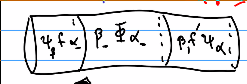
\includegraphics[width=0.8\linewidth]{mcyl}
        \caption{Picture of $\Phi_i$}%
        \label{fig:}
    \end{figure}
    Here, $\psi_{\alpha_-}$ is a homotopy from $\alpha \alpha_-$ to $\mr{id}_{X'}$ and $\psi_{\beta}$ is defined analogously. Then the three components are first $\beta_- f' \psi_{\alpha_-}$, then $\beta_- \Phi \alpha_-$, and finally $\psi_{\beta} f \alpha_-$.

    Finally, it is easy to check that the piecewise homotopies agree at the boundaries.
\end{proof}

\begin{rmk}
    This is \textbf{not} a true inverse! However, they are homotopic.
\end{rmk}

The mapping cylinder generalizes to a \textit{double mapping cylinder} $Z(f,g)$ for spans $B \xleftarrow{g} A \xrightarrow{f} C$. 

\begin{lem}
    If the diagram
    \begin{equation}
    \begin{tikzcd}
        A \arrow{r}{f} \arrow{d}{g} & B \arrow{d} \\
        C \arrow{r} & X
    \end{tikzcd}
    \end{equation}
    homotopy commutes, then we can fit the mapping cylinder $Z(f,g)$ into the diagram with an arrow $Z(f,g) \to X$. However, this arrow depends on the choice of homotopy.
\end{lem}

\begin{defn}
    $X$ is a \textit{homotopy pushout}  of the diagram in the previous lemma if $Z(f,g) \to X$ is a homotopy equivalence.
\end{defn}

Note this is \textbf{not} unique in $\ms{Top}$, but is unique in $\ms{hTop}$.

\begin{exm}
    Consider the projections $X \gets X \times Y \to Y$. Then a homotopy pushout is the join $X * Y$.
\end{exm}

\begin{exm}
    The homotopy pushout of $* \gets X \to *$ is the \textit{unreduced suspension} $\Sigma' X$. 
\end{exm}

Then recall the reduced suspension $\Sigma X = \Sigma' X / * \times I$. Then this is related to another familiar construction. The key fact is
\[ F^0(\Sigma X, Y) = \{ \gamma: X \times I \to Y \mid \gamma(x,t) = g \text{for all $t$}, \gamma(x,0) = \gamma(x,1) = y = F^0(X, \Omega Y). \]
This tells us that the suspension and loop space functors are adjoint.
Also note that concatenation makes $\Omega Y$ into an \textit{H-space} , which is a monoid in $\ms{hTop}^0$. 

Concretely, concatenation is \textit{homotopy associative} and $y \in Y$ is a (pointed) homotopy unit. Therefore, $[X, \Omega Y]$ is a group. To see this from the point of $[\Sigma X, Y]$, we see that $\Sigma X$ is a \textit{comonoid}. The map $\Sigma X \to \Sigma X \vee \Sigma X$ is simply given by collapsing $X \times \{ 1/2 \}$.  

Consider the diagram
\begin{equation}
\begin{tikzcd}
    X \arrow{r}{f} \arrow{d} & Y \arrow{d} \\
    * \arrow{r} & Y/X.
\end{tikzcd}
\end{equation}
Then we have a series of maps $F^0(Y/X,B) \to F^0(Y,B) \to F^0(X,B)$. Then define $C(f) = Z(f) / X \times \{0 \} \cup \{x\} \times I$. We now have a map $X \xrightarrow{f} Y \to C(f)$. We will use the mapping cone to replace the quotient.

\begin{lem}
    The sequence $[C(f),B]^0 \to [Y,B]^0 \xrightarrow{f} [X,B]^0$ is exact at $[Y,B]^0$ for any based space $B$. In other words, the composition sends $[C(f),B]$ to the constant map $X \to B$.
\end{lem}

\begin{proof}
    Given a map $Y \to B$ and a homotopy $\Phi$, construct $C(f) \to B$ by using the construction for the double mapping cylinder.
\end{proof}

Now we can extend to the left by considering the map $C(f) \to \Sigma X$ given by collapsing $Y$. This gives us a diagram
\[ X \xrightarrow{f} ^ \to C(f) \to \Sigma X \xrightarrow{\Sigma f} \Sigma Y \to C(\Sigma f) \to \cdots \]
Finally, we only need to check that $Y \to C(f) \to \Sigma X$ and $C(f) \to \Sigma X \to \Sigma Y$ are coexact. To check this, note that $\Sigma X$ is homotopy equivalent to $C(Y \hookrightarrow C(f))$ and the other one is easy.

\begin{cor}
    For each space $B$, we have an exact sequence
    \[ \cdots \to [\Sigma C(f),B]^0 \to [\Sigma Y, B]^0 \to [\Sigma X,B]^0 \to [C(f),B]^0 \to [Y,B]^0 \to [X,B]^0. \]
    If we extend to the left, we obtain \textit{abelian groups} because the double loop space is a commutative H-space. 
\end{cor}

\section{Homotopy Pullbacks}%
\label{sec:homotopy_pullbacks}

Now we will dualize everything and look for
\[ [B,X]^0 \to [B,Y]^0 \to [B,?]^0 \to \cdots \]
The cone is a homotopy pushout, so we will define an analogous homotopy pullback for
\begin{equation}
\begin{tikzcd}
    & * \arrow{d} \\
    x \arrow{r} & Y.
\end{tikzcd}
\end{equation}
This will be known as the \textit{homotopy fiber}. In the usual category of $\ms{Top}$, this is the actual fiber. To do this, we will replace the point by $F Y = \{ \gamma: I \to Y \mid \gamma(0) = y \}$. This is contractible by retracting every path to $y$, so we will define $F(f)$ to be the pullback of the above diagram.

\begin{lem}
    The sequence $[B,F(f)]^0 \to [B,X]^0 \to [B,Y]^0$ is exact.
\end{lem}

Proof is given by using the interval direction to construct the map from $B$ to $F(f)$. In more words, we interpret a homotopy $B \times I \to Y$ as a map $B \to FY$. In addition, this lemma constructs a fiber sequence
\[ \cdots \to \Omega F(f) \to \Omega X \to \Omega Y \to F(f) \to X \to Y, \]
which yields a long exact sequence
\[ \cdots \to [B, \Omega Y]^0 \to [B,F(f)]^0 \to [B,X]^0 \to [B,Y]^0. \]

\section{Fibrations and Cofibrations}%
\label{sec:fibrations_and_cofibrations}

Assume that $X$ is Hausdorff. 

\begin{defn}
    A map $ A \xrightarrow{i} X$ is a \textit{cofibration} if any diagram
    \begin{equation}
    \begin{tikzcd}
        A \arrow{r} \arrow{d}{i} & Y^I \arrow{d}{e_0} \\
        X \arrow{r} \arrow[dashrightarrow]{ur} & Y
    \end{tikzcd}
    \end{equation}
    admits a lift. This is called the \textit{homotopy extension property}. 
\end{defn}

In other words, we can extend diagrams of the form
\begin{equation}
\begin{tikzcd}
    A \arrow{rr}{a \times \{0\}} \arrow{dd}{i} & & A \times I \arrow{dd} \arrow{dl} \\
                                               & Y & \\
    X \arrow{rr} \arrow{ur} & & X \times I. \arrow[dashrightarrow]{ul}
\end{tikzcd}
\end{equation}

\begin{prop}
    Pushouts preserve cofibrations. In other words, for a pushout
    \begin{equation}
    \begin{tikzcd}
        A \arrow{r}{f} \arrow{d}{j} & B \arrow{d}{J} \\
        X \arrow{r} & Y,
    \end{tikzcd}
    \end{equation}
    if $j$ is a cofibration, then so is $J$.
\end{prop}

\begin{proof}
    We will diagram chase. We construct the full diagram
    \begin{equation}
    \begin{tikzcd}
        A \arrow{rrrr} \arrow{dddd}{j} \arrow{dr} & & & & A \times I \arrow{dl} \arrow{dddd} \\
        & B \arrow{rr} \arrow{dd}{J} & & B \times I \arrow{dl} \arrow{dd} \\
        & & Z \\
        & Y \arrow{rr} \arrow{ur} & & Y \times I \arrow[dashrightarrow]{ul} \\
        X \arrow{ur} \arrow{rrrr} & & & & X \times I. \arrow{ul}
    \end{tikzcd}
    \end{equation}
    Then the map $X \times I \to Z$ exists by cofibrations, and then the arrow $Y \times I \to Z$ exists because $Y \times I$ is a pushout.
\end{proof}

This proof is completely formal, and we had no idea what is going on.

\begin{exm}
    $ \{ 0 \} \subset I$ is a cofibration. To see this, note that we can identify $I$ with two sides of the square, and the retract the square onto the two sides of the interval. Note that two sides of the square form the mapping cylinder of $0 \in I$.
\end{exm}

\begin{prop}
    $A \subset X$ is a cofibration if and only if it satisfies the homotopy extension property for $Z(i)$.
\end{prop}

\begin{proof}
    Suppose the lift $X \to Z(i)^I$ exists. Then this induces a map $Z(i) \to Y$. Then we can map $X \times I \to Z(i)$ and compose.
\end{proof}

\begin{prop}
    $A \subset X$ is a cofibration if and only if it is a neighborhood deformation retract. This is defined by $\nu \colon X \to I$ and $\psi \colon X \times I \to X$ wuch that
    \begin{enumerate}
        \item $\nu^{-1}(0) = A$.
        \item $\psi(a,t) = a$ for all $a \in A, t \in I$.
        \item If $\nu(x) < 1$, then $\psi(x,1) \in A$.
        \item $\psi(x,0) = x$.
    \end{enumerate}
\end{prop}

The proof uses the previous criterion. The point is to deformation retract $X \times I$ onto $Z(i)$.

We want to be able to compute things, and we will start with cofibrant replacements. Because $\{ 0 \} \subset I$ is a cofibration, so is $X \to Z(f)$ for any $f \colon X \to Y$. Then inclusion $Y \hookrightarrow Z(f)$ is a homotopy equivalence, so we can factor $f$ into a homotopy equivalence and a cofibration. Functoriality of the mapping cylinder was discussed previously.

\begin{quest}
    Let $f \colon X \to Y$ be a homotopy equivalence such that $X,Y$ are equipped with extra structure. Can the homotopy equivalence be made compatible with this extra structure?
\end{quest}

\begin{exm}
    Suppose $X,Y$ live under a space $K$. Then we can define a homotopy equivalence under $K$.
\end{exm}

\begin{prop}
    If $i \colon K \to X,j \colon K \to Y$ are cofibrations, then $f \colon X \to Y$ is a homotopy equivalence in $\ms{Top}$ if and only if it is a homotopy equivalence in $\ms{Top}^K$.
\end{prop}

\begin{proof}
    Let $g$ denote the homotopy inverse of $f$. Then consider the space $(X, g \circ j)$ under $K$. If we fix a homotopy $gf \sim \mr{id}$, this induces an isomorphism $\varphi^{\sharp} \colon [(X,i), (X,gfi)]^K \to [(X,i), (X,i)]^K$. This is done by extending to $X \times I \to K$ by the homotopy extension property.

Note that $\varphi^{\sharp}$ is a transport map. If $i \colon A \to X$ is a cofibration and $\varphi \colon A \times I \to Y$ is a homotopy. 
\end{proof}

\begin{prop}
    Let $A \xrightarrow{i} X$ and $B \xrightarrow{j} Y$ be cofibrations. Then if $f \colon A \to B$ and $F \colon X \to Y$ make the diagram commute, then $(f, F)$ is a homotopy equivalence of pairs if and only if $f$ and $F$ are both homotopy equivalences.
\end{prop}

If we dualize everything, we replace $Y^I$ by $X \times I$. Now we consider a map $p \colon E \to B$.

\begin{defn}
    A map $p \colon E \to B$ is a \textit{Hurewicz fibration} if all diagrams of the form
    \begin{equation}
    \begin{tikzcd}
        X \arrow{r} \arrow{d} & E \arrow{d}{p} \\
        X \times I \arrow{r} \arrow[dashrightarrow]{ur} & B
    \end{tikzcd}
    \end{equation}
    admit a lift. This is called the \textit{homotopy lifting property}.  
\end{defn}

\begin{defn}
    A map $p \colon E \to B$ is a \textit{Serre fibration} if it satisfies the homotopy lifting property for all cubes. 
\end{defn}

\begin{lem}
    Pullbacks preserve fibrations.
\end{lem}

The test object we will use to study fibrations is the pullback $W(p) = \{ (e,w) \mid p(e) = w(0) \} \subset E \times B^I$.

\begin{prop}
    $W(p) \to E$ is a hommotopy equivalence. In addition, $p$ is a fibration if and only if it has the homotopy lifting property for $W(p)$.
\end{prop}

Now, let $X \xrightarrow{f} Y$ be an arbitrary map. Then we can factor $X \to W(f) \to Y$ as a fibration and a homotopy equivalence.

\begin{exm}
    All covering maps are fibrations. Also, if $A \to X$ is a cofibration, the dual $B^X \to B^A$ is a fibration. Similarly, if $E \to B$ is a fibration, then so is $Z^E \to Z^B$.
\end{exm}

Now suppose $f \colon X \to Y$ is a homotopy equivalence of spaces over $B$. Then if $p \colon X \to B$ and $q \colon Y \to B$ are fibrations, $f$ is a homotopy equivalence in $\ms{Top}$ if and only if it is a homotopy equivalence in $\ms{Top}_B$.

\section{Homotopy Groups}%
\label{sec:homotopy_groups}

Let $X$ be a based space.

\begin{defn}
    The $n$-th \textit{homotopy group}  of $X$ is 
    \[ \pi_n(X,*) = [(I^n, \partial I^n), (X,*)] \cong [I^n / \partial I^n, X]^0. \]
\end{defn}

\begin{defn}
    Given a pair $(X,A)$ of based spaces, the $n$-th \textit{relative homotopy group} is
    \[ \pi_{n+1}(X,A,*) = [(I^n, \partial I^{n+1}, \mc{J}^n), (X, A, *)] \]
    where $\mc{J}^n = \partial I^n \times I \cup I^n \times \{0 \}$. Here, the source triple is homotopy equivalent to $(D^{n+1}, S^n, *)$.
\end{defn}

We will attempt to develop some tools to compute homotopy groups. Let $F(X,A) = \qty{w \colon I \to X \mid w(0) = *, w(1) \in A}$. By splitting $(F(I^{n+1}, \partial I^{n+1}, \mc{J}), (x, A, *)) \cong F((I^n, *), (F(X,A), *))$ and using the suspension-loop adjunction, we obtain
\[ \pi_n(X, *) \cong \pi_{n-1}(\Omega X, *) \cong \cdots \cong \pi_1(\Omega^n X, *). \]
Therefore the relative homotopy group is the set of components of the $n$-th loop space of $F(X,A)$. The loop space appears in the fiber exact sequence, and $F(X,A)$ is simply the homotopy fiber of $A \to X$, so if we set $B = S^0$, we obtain from the long exact sequence
\[ \cdots \to \Omega(F(X,A)) \to \Omega A \to \Omega X \to F(X,A) \to A \to X \]
the exact sequence of homotopy groups
\[ \cdots \to \pi_0(\Omega F(X,A)) \to \pi_0 \Omega A \to \pi_0 \Omega X \to \pi_0(F(X,A)) \to \pi_0(A) \to \pi_0(X) \]
which becomes
\[ \cdots \to \pi_2(X,A) \to \pi_1(A) \to \pi_1(X) \to \pi_1(X,A) \to \pi_0(A) \to \pi_0(X). \]
\begin{warn}
    The relative homotopy group is \textbf{not} the same as the homotopy group of the quotient. 
\end{warn}

Here, we were very sloppy with basepoints and all of our homotopy groups should have carried basepoints. Last time, we showed that a homotopy $K \times I \xrightarrow{\varphi} X$ induces a transport map
\[ (A, i), (X, \varphi_0)^K \to [(A,i), (X, \varphi_1)]^k \]
if $K \to A$ is a cofibration. Applying this to $K = \mr{pt}, A = S^n$, we obtain a transport $\pi_n(X, *) \to \pi_n(X, *')$.

\begin{prop}
    The assignment $* \to \pi_n(X, *)$ defines a functor $\Pi X \to \ms{Set}$. If $n \geq 1$, the target of the functor can be replaced with $\ms{Grp}$.
\end{prop}

\begin{cor}
    \begin{enumerate}
        \item Up to some isomorphism, the $n$-th homotopy group is invariant of the choice of basepoint. The choice is not canonical unless $\pi_1$ acts trivially.
        \item If $f \colon X \to Y$ is a homotopy equivalence, then the induced map on homotopy groups is an isomorphism.
        \item $\pi_1(X,*)$ acts naturally on $\pi_n(X,*)$.
    \end{enumerate}
\end{cor}

Now suppose $E \xrightarrow{\pi} B$ is a fibration. Then the homotopy fiber is homotopy equivalent to the actual fiber $F$, so the relative homotopy groups of $F$ in $E$ are isomorphic to the homotopy groups of the base. To construct an explicit map $\pi_k(E,F,*) \gets \pi_j(B,*)$, we begin with a sphere in $B$. Then we use the homotopy lifting property to obtain a disc in $E$ with boundary in $E$.

It is easy to see the following:
\begin{enumerate}
    \item If $X$ is contractible, then $\pi_i(X,*) = 0$ for all $i > 0$.
    \item The argument we gave for $\pi_1(S^n, *)$ for $n \geq 2$ also shows that $\pi_1(S^n, *) = 0$ for $i < n$. To see this, consider $S^i \xrightarrow{f} S^n = \R^n \cup \infty$. First, we can find a homotopic map $f'$ which is smooth and transverse to $\infty$. This implies the image lies in $\R^n$ if $i < n$, so $f'$ is nullhomotopic because $\R^n$ is contractible.
    \item If $\wt{X} \to X$ is a covering map, then $\pi_i(\wt{X}, \wt{x}) \to \pi_i(X,x)$ is an isomorphism for $i > 2$. To see this, we use the lifting property for maps
        \begin{equation*}
        \begin{tikzcd}
            & \wt{X} \arrow{d} \\
            S^n \arrow{r} \arrow[dashrightarrow]{ur} & X
        \end{tikzcd}
        \end{equation*}
        because $0 = \pi_1(S^n) \to \pi_1(X)$. 

        As an example, this allows us to compute $\pi_1(S^1) = \Z$, and $\pi_i(S^1) = 0$ for $i > 1$ because the universal cover $\R$ is contractible.
    \item Consider the Hopf fibration $S^1 \to S^3 \to S^2$. Applying the long exact sequence, we have
        \[ 0 = \pi_2(S^3) \to \pi_2(S^2) \to \pi_1(S^1) \to \pi_1(S^3) = 0 \]
        and observe that $\pi_2(S^2) = \Z$.
\end{enumerate}

We would naively expect that $\pi_i(S^n) = 0$ for $i > n$, but this is incorrect. However, it is true that $\pi_n(S^n) = \Z$. For higher homotopy groups, it is easy to see that an analog of the Seifert-van Kampen theorem does not hold. If we write $S^2 = D^2 \cup D^2$, then $D^2$ and $S^1$ both have trivial $\pi_2$, but $S^2$ does not.

What does hold is Blakers-Massey. Assume that $Y = Y_1 \cup Y_2$, where the $Y_i$ are open. Suppose that $Y_0 = Y_1 \cap Y_2$ is nonempty. Then we have a map
    \[ \pi_1(Y_2, Y_0) \to \pi_i(Y, Y_1) \]
    called the \textit{excision}. 

\begin{thm}[Blakers-Massey]
    Assume that $(Y_1, Y_0)$ is $p$-connected and $(Y_2, Y_0)$ is $q$-connected. Then excision is an isomorphism in degree $i < p+q$ and surjective in degree $i = p+q$. This means that excision is $(p+q)$-connected as a map of pairs.
\end{thm}

Note that a pair $(X,A)$ is $p$-connected if $\pi_1(X,A,*) = 0$ for $0 \leq i \leq p$. This is equivalent to $\pi_i(A) \simeq \pi_i(X)$ for $i < p$ and $\pi_p(A) \twoheadrightarrow \pi_p(X)$.

Now we can prove that $\pi_n(S^n) = \Z$. First consider $n = 2$. Then we have a long exact sequence
\[ \cdots \to \pi_2(D^2, S^1) \to \pi_1(S^1) \to \pi_1(D^2) \to \cdots \]
and we see that $\pi_2(D^2, S^1) \cong \Z$. We now apply excision for $\pi_2(D^2_-, S^1) \to \pi_2(S^2, D^2_+) \cong \pi^2(S^2) \cong \Z$. To see that excision is an isomorphism, use the Hopf fibration.

In the next dimension, we use the same computation to see that $\pi_3(D^3, S^2) \cong \Z$ and the pairs $(D^3_+, S^2), (D^3_-, S^2)$ are $2$-connected. Then the map $(D^3_+, S^2) \to (S^3, D^3_-)$ is $4$-connected, so $\pi_3(S^3) \cong \pi_3(S^3, D^3_-) \cong \pi_3(D^3, S^2) \cong \Z$.

\begin{thm}
    If $Y_1 \to Y$ and $Y_2 \to Y$ are $p$ and $q$-connected, then $F(Y_1, Y_1, Y_0) \subset F(Y_1, Y, Y_2)$ is $p + q - 1$ connected. Here, $F(Y_1, Y_1, Y_0)$ are paths $w \colon I \to Y$ such that $w(0) \in Y$, $w(1) \in Y_0$.
\end{thm}

This implies Blakers-Massey by taking the fiber over $0$. Note that the homotopy fiber of $Y_0 \to Y_1$ is 
\begin{equation*}
\begin{tikzcd}
    F(*, Y_1, Y_0) \arrow{d} \arrow{r} & F(*, Y, Y_2) \arrow{d} \\
    F(Y_1, Y_2, Y_0) \arrow{r} \arrow{d}{ev_0} & F(Y_1, Y, Y_2) \arrow{d}{ev_0} \\
    Y_1 \arrow{r}{=} & Y_1.
\end{tikzcd}
\end{equation*}
Then using the long exact sequence of homotopy groups, we obtain the desired result.

Now consider the special case $Y = D^{q+1} \cup_{S^q} Y_0 \cup_{S^p} D^{p+1}$. This is the pushout
\begin{equation*}
\begin{tikzcd}
    S^q \sqcup S^p \arrow{d} \arrow{r} & D^{q+1} \cup D^{p+1} \arrow{d} \\
    Y_0 \arrow{r} & Y.
\end{tikzcd}
\end{equation*}
and looks something like
\begin{figure}[H]
    \centering
    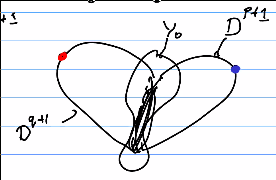
\includegraphics[scale=0.8]{attachcell.png}
    \caption{Attaching two cells to $Y_0$}%
    \label{fig:attachcell}
\end{figure}
The key idea is that if $I^n \xrightarrow{\sigma} F(Y)$ is a family of paths, then generically, the subfamily $Q \subset  I^n$ of paths which intersect the origin in $D^{q+1}$ has dimension $n-q$. To see this, appeal to the fact that locally $D^{q+1}$ is a manifold and then use Sard's theorem. If a path is not in $Q$, then we can retract it to $F(Y_1, Y_1, Y_0)$ ``radially'' in $D^{q+1}$. Such a path lies in $D^{p+1} \cup Y_0 \cup D^{q+1} \setminus 0$.

If our path lies in $Q$, then we have a dimension $n-q-p$ locus passing through $0 \in D^{p+1}$. If $n < q+p$, then the dimension is negative, so it is empty. Thus generically, every path misses either $0 \in D^{p+1}$ or $0 \in D^{q+1}$. Then we can retract $Q$ to $F(Y_0, Y_2, Y_2)$. But then we can move the basepoint along $Y_2$ back to $Y_0$, so we retract to
\[ Y_0 \to F(Y_0, Y_0, Y_0) \subset F(Y_1, Y_1, Y_0). \]
We will ignore the details needed to make this precise. To handle the general case, we simply need to consider the case where an arbitrary number of cells are attached and then use CW approximation.

Here are some applications of Blakers-Massey:
\begin{cor}
    Say $A \subset X$ is a cofibration. Then suppose $A$ is $m$-connected and $(X,A)$ is $n-1$ connected. Then $(X,A) \to (X/A, *)$ is $n+m-1$ connected.
\end{cor}

\begin{proof}
    Take the mapping cylinder $Z(f)$. Cover this by $C(A) \cup_A X$. Then $A$ is $m$-connected if and only if $A \to CA$ is $m$-connected. Using the fact that $(X,A)$ is $n-1$ connected, we use Blakers-Massey to obtain the desired result.
\end{proof}

\begin{cor}[Freudenthal]
    Assume $X$ is well-pointed and $n-1$ connected. Then $\pi_i(X) \to \pi_{i+1}(\Sigma X)$ is an isomorphism for $i \leq 2n-2$ and is surjective for $i = 2n-1$.
\end{cor}

\begin{proof}
    Note that $\Sigma X = C_+X \cup_X C_-X$. The only thing we need to check is that the map from Blakers-Massey is the same as the suspension map.
\end{proof}

\begin{cor}
    If $X$ is $n$-connected and $Y$ is $m$-connected, then $X \wedge Y$ is $n+m+1$ connected.
\end{cor}

\begin{proof}
    Note that $X \wedge Y = X \times Y / X \vee Y$. We need to understand $\pi_{i+1}(X \times Y, X \vee Y)$. But then $\pi_i(X \times Y) = \pi_i(X) \oplus \pi_i(Y)$, so 
    \[ \pi_i(X \vee Y) \cong \pi_i(X) \oplus \pi_i(Y) \oplus \pi_{i+1}(X \times Y, X \vee Y). \]
    Then using excision to compute $\pi_i(X \vee Y) = \pi_i(X) \oplus \pi_1(Y)$ in the range, we obtained the desired result.
\end{proof}

In the text, there is more discussion of the homotopy groups of $\R\P^n$, which has $S^n$ as its universal cover. Then if we take the colimit of
\[ \R\P^1 \subset \R\P^2 \subset \cdots \]
and obtain $\R\P^{\infty}$, this has trivial homotopy. We can prove this by noting that $S^{\infty}$ is contractible.

We can also consider the action of $O(n)$ on $S^{n-1}$. We then obtain a fiber sequence $O(n-1) \to O(n) \to S^{n-1}$. Then we can use induction to compute the difference between $\pi_i(O(n-1))$ and $\pi_i(O(n))$. For $i \leq n-2$, the groups are isomorphic. Then we consider the colimit
\[ O(n-1) \hookrightarrow O(n) \hookrightarrow O(n+1) \hookrightarrow \cdots \]
to obtain the group $O(\infty)$ with periodic homotopy groups $\Z_2, \Z_2, 0, \Z, 0, 0, 0, \Z$ by Bott periodicity. We can do the same computation for the unitary group.

\chapter{CW Complexes and Homology}%
\label{cha:changing_spaces}

\section{$K$-Spaces}%
\label{sec:_k_spaces}

Recall that whenever $X,Y$ are locally compact, then we have the adjunction
\[ F(X \times Y, Z) \to F(X, F(Y, Z)). \]
We want this to always hold, so we will need to study infinite complexes. For example, an infinite wedge of circles is not locally compact. Our solution will be to change the topology on $F$ and on $X$.

\begin{defn}
    $X$ is a \textit{$K$-space} if, for all $A \subset X$, if $f^{-1}(A)$ is closed for all $f \colon K \to X$ with $K$ compact Hausdorff, then $A$ is closed.
\end{defn}

Now we define a functor $K \colon \ms{Top} \to \ms{Top}$. Here, $KX$ is $X$ as a set with closed sets those such that $f^{-1}(A)$ closed for all $f \colon K \to X$ continuous in the original topology. Because $KX$ has more closed sets than $X$, then we have a natural transformation between $K$ and the identity.

\begin{prop}
    $X$ is a $K$-space if and only if the following hold: Any map $f \colon X \to Y$ is continuous if and only if $K \to X \to Y$ is continuous for all $K \to X$ with $K$ compact Hausdorff.
\end{prop}

Let $\ms{kTop} \subset \ms{Top}$ be the full subcategory of $K$-spaces.

\begin{thm}
    Products exists in $\ms{kTop}$.
\end{thm}

\begin{thm}
    We have the adjunction
    \[ kF(X \times Y, Z) \cong kF(X, kF(Y, Z)). \]
\end{thm}

We did all of this because non locally compact spaces show up relative naturally. 

\section{Simplicial Complexes}%
\label{sec:simplicial_complexes}

A \textit{simplicial complex} is a set $V$ with a collection $S$ of finite subsets $\sigma \subset V$ such that $\sigma \setminus \{v \} \in X$ for all $v \in \sigma$.

Letting $\Delta(\sigma) = \qty{\sum_{v \in \sigma} i_V = 1} \subset I^{v}$, then we have natural maps $\Delta(\sigma \setminus \{v\}) \subset \Delta(\sigma)$.

\begin{defn}
    The \textit{geometric realization} $\abs{K}$ of a simplicial compex $K$ is the space
    \[ \bigsqcup_{\sigma \in S} \Delta(\sigma) / \sim \subset I^V \]
    where $\sim$ is the equivalence defined by the maps above.
\end{defn}

If we have a homeomorphism $\abs{K} \cong X$, then this is said to be a \textit{trianglation} of $X$. All smooth manifolds can be triangulated.

This is very rigid, which is bad for homotopy theory, so we give an alternative viewpoint. Let $K^n = (V, S^n)$, where $S^n$ is the subsets of size at most $n+1$. This is called the \textit{$n$-skeleton}, so the geometric realization $\abs{K^n}$ induces the simplices of dimension at most $n$. Then we have a pushout
\begin{equation*}
\begin{tikzcd}
    \bigsqcup_{\sigma \in S^{n+1} \setminus S^n} \partial \Delta(\sigma) \arrow{r} \arrow{d} & \abs{K^n} \arrow{d} \\
    \bigsqcup \Delta(\sigma) \arrow{r} & \abs{K}^{n+1}.
\end{tikzcd}
\end{equation*}

\begin{lem}
    $\abs{K} = \operatorname{colim}_n \abs{K}^n$.
\end{lem}
To prove this, we check that the topology agrees. Unfortunately, the maps from simplices are too rigid, so to derigidify, we will relax the notion of the attaching maps.

\section{CW complexes}%
\label{sec:cw_complexes}

\begin{defn}
    A CW decomposition of a space $X$ is a filtration $X = \operatorname{colim} X_i \ni X_0 = \mr{pt}$ such that we have pushouts
    \begin{equation*}
    \begin{tikzcd}
        \bigsqcup_{i \in C_n} S_i^{n-1} \arrow{r}{\phi} \arrow{d} & X_{n-1} \arrow{d} \\
        \bigsqcup_{i \in C_n} D_i^n \arrow{r} & X_n.
    \end{tikzcd}
    \end{equation*}    
\end{defn}

\begin{rmk}
    Let $E^n = D^n \setminus S^n$. We obtain a decomposition as a set
    \[ X = \bigsqcup_{\lambda \in \bigcup_n C_n} e_{\lambda} \]
    where $e_{\lambda}$ is the image of $E_i^n$ in $X$.
\end{rmk}

A key property is that if $K \subset X$ is compact, then $K$ intersects only finitely many cells. To see this, note that $K \subset X^n$ for some $n$. Then $K$ lies in an infinite union of disks, so it must intersect finitely many of them.

\begin{rmk}
    The abbreviation CW stands for closure-finite (C) and weak topology (W).
\end{rmk}

\begin{defn}
    A \textit{CW decomposition} of a pair $(X,A)$ is a filtration $X = \mr{colim} X_i$ where $X_{-1} = A$ and $X_n$ is given as a pushout
    \begin{equation*}
    \begin{tikzcd}
        \bigsqcup_{i \in C_n} S_i^{n-1} \arrow{r} \arrow{d} & X_{n-1} \arrow{d} \\
        \bigsqcup_{i \in C_n} D_i^n \arrow{r} & X_n.
    \end{tikzcd}
    \end{equation*}
    Here, the cell attachment happens in dimension $n$.
\end{defn}

If $A = \emptyset$, we have a CW decomposition of $X$. Then we say that $\dim X \leq n$ if all cells have at most that dimension. Now there are two ideas for working with CW-complexes.

\begin{enumerate}
    \item Suppose $A \xrightarrow{f} Y$ is a map. If $(X,A)$ is a relative CW complex, we want to extend $f$ to $F \colon X \to Y$. The obstruction is as follows. Say we only have one cell. Then $S^{n-1} \to A \to Y$ defines an element of $\pi_{n-1}(Y)$, and this vanishes if and only if an extension exists. If $X$ has more cells, then proceed by induction (we have a sequence of obstructions, and we need them all to vanish).
    \item (Cellularity) Say that $(Y,B)$ is $n$-connected. If $X$ is a CW complex and $f \colon X \to Y$ is a map with $\dim X < n$, then $f$ is homotopic to some $f'$ with $f'(X) \subset B$.

        To prove this, use induction. We know that $Y,B$ have the same components, so we may deform $f$ so that $X^0$ maps to $B$ (use the transport with $X^0 \subset X$ a cofibration). Then each $1$-cell of $X$ determines an element of $\pi_1(Y,B) = 0$, so we can make $X^1$ map to $B$.
\end{enumerate}

Here are some consequences:
\begin{enumerate}
    \item If $\pi_i(Y) = 0$ for all $i \geq n$ and $(X,A)$ is a relative CW complex which is $(n+1)$-connected, then $[X,Y] \simeq [A,Y]$. Note all obstructions to the extension vanish.
    \item Say $f \colon B \to Y$ is an $n$-connected map. If $X$ is a CW complex, then $[X,B] \to [X,Y]$ is an isomorphism if $\dim X < n$ and a surjection if $\dim X = n$. Here, use the mapping cylinder to reduce to the case of an inclusion and then note that obstructions vanish.
\end{enumerate}

\begin{rmk}
    Conditions on $\pi_i$ of the target are in some sense dual to the source having no cell in a given dimension (replace this by vanishing cohomology).
\end{rmk}

We can now let $n = \infty$ (i.e.~a weak homotopy equivaence).

\begin{prop}
    A map $f \colon X \to Y$ of CW complexes is a homotopy equivalence if and only if $f_* \colon \pi_i(X) \to \pi_i(Y)$ is an isomorphism for all $i$.
\end{prop}

\begin{proof}
    For any $n$-connected $Z$, we have an isomorphism $f_* \colon [Z,X] \to [Z,Y]$. Then if we let $Z = Y$, note that $[Y,X] \to [Y,Y]$ and choose an inverse fo $\mr{id}_Y$. Alternatively, this is just the Yoneda Lemma.
\end{proof}

\begin{rmk}
    If $\dim X = \dim Y \leq k$, then we only need to check $\pi_i$ for $i \leq k$.
\end{rmk}

\begin{rmk}
    If it \textbf{not true} that CW complexes are determined up to homotopy equivalence by their homotopy groups. The counterexample is $X = BU$ and $Y = \bigvee K(\Z, 2i)$, but to prove this, we need to use cohomology. 
\end{rmk}

\begin{prop}
    For any space $Y$ there exists a CW complex $X$ and a map $X \to Y$ which is a weak homotopy equivalence. This is not a homotopy equivalence in general (see the pseudocircle from the homework), but for $Y$ a manifold, it is a homotopy equivalence.
\end{prop}

\begin{proof}
    By induction on $n$, we want $X^n \to $ which is $n$-connected. Using the mapping cylinder, we can assume that $X^n \hookrightarrow Y$. Consider $\pi_{n+1}(Y, X^n)$. Define $X^{n+1}$ as the result of attaching $n+1$ discs to $X^n$ indexed by a basis of this group. Extend the map to $X^{n+1}$ and use the long exact sequence to see that $X^{n+1} \to Y$ is $n+1$ connected. To see that we can extend, note that we have the diagram
    \begin{equation*}
    \begin{tikzcd}
        S^n \arrow{r} \arrow{d} & X^n \arrow{r} \arrow{d} & Y \\
        D^{n+1} \arrow{r} & X^{n+1}. \arrow[dashrightarrow]{ur}
    \end{tikzcd}
    \end{equation*}
    Then we can extend from the disk by using the associated element of $\pi_{n+1}(Y,X)$. Now we have a diagram
    \begin{equation*}
    \begin{tikzcd}
        \pi_{n+1}(X^n) \arrow{r} \arrow{d}{=} & \pi_{n+1}(X^{n+1}) \arrow{d} \arrow{r} & \pi_{n+1}(X^{n+1},X^n) \arrow{r} \arrow{d} & \pi_n(X^n) \arrow{d}{=} \\
        \pi_{n+1}(X^n) \arrow{r} & \pi_{n+1}(Y) \arrow{r} & \pi_{n+1}(Y, X^n) \arrow{r} & \pi_n(X^n).
    \end{tikzcd}
    \end{equation*}
    Then we can show that the left middle arrow is surjective, and then by surjectivity of the whole diagram, we see that the desired arrow is surjective.
\end{proof}

Now we give a useful computation. Suppose that $\pi_i(Y) = 0$ for all $i > n \geq 2$ and that $X$ is a $(n-1)$-connected CW complex. Then $[X,Y] \cong \Hom(\pi_n(X), \pi_n(Y))$.

Surjectivity is easy (use lemma about $[X,Y] \cong [A,Y] \ldots$). To prove injectivity, we sill reduce to $X$ being the cone of $\bigvee S^n \to \bigvee S^n$, by assumption, $n \geq 2$, so $X$ is a suspension. Then we have a sequence of groups
\begin{equation*}
\begin{tikzcd}
    { [A,Y] }^0 \arrow{d}{\sim} & { [B,Y] }^0 \arrow{l}{\phi^*} \arrow{d}{\sim} & { [X,Y] }^0 \arrow{d} \arrow{l} & { [\Sigma A, Y] }^0 \arrow{l} \arrow{d} \\
    \Hom(\pi_n(A), \pi_n(Y)) & \Hom(\pi_n(B), \pi_n(Y)) \arrow{l} & \Hom(\pi_n(X), \pi_n(Y)) \arrow{l} & 0. \arrow{l}
\end{tikzcd}
\end{equation*}
Then we use Blakers-Massey to prove exactness and then obtain the desired result.

\section{Eilenberg-Maclane Spaces}%
\label{sec:killing_homotopy_groups}

Now recall that the universal cover $\wt{Y} \to Y$ satisfies 
\begin{enumerate}
    \item $\pi_1(\wt{Y}) = 0$
    \item $\pi_i(\wt{Y}) \cong \pi_1(Y)$ if $i > 1$.
\end{enumerate}
We want to generalize this to a general procedure ($n$-connected cover), which will be a fibration, but not a covering space.

Given a space $Y$ and integer $n$, let $Y[n]$ be the result of attaching cells to kill $\pi_i$ for $i \geq n$. This means that $\pi_i(Y_m) = 0$ for $i \geq n$ and $\pi_i(Y_m) = \pi_i(Y)$ otherwise.

\begin{exm}
    There exists a space $S^n[n+1]$ with $\pi_i = \begin{cases}
        \Z & i = n \\
        0 & \text{otherwise}
    \end{cases}$.
\end{exm}

Let $\pi$ be a group and $n \in \N$. 
\begin{defn}
    A CW complex $X$ is a $K(\pi, n)$ if
    \[ \pi_i(X) = \begin{cases}
        0 & i \neq n \\
        \pi & i = n
    \end{cases}. \]
\end{defn}

The key fact is that $K(\pi, n)$ is unique up to homotopy equivalence by a previous lemma. To show existence, we will present $\pi$ as a quotient of $F^I \to F^J$ (free if $n=1$, free abelian if $n \geq 2$). Then consider the cone of $\bigvee_I S^n \to \bigvee_J S^n$. The $\pi_n$ is correct by Blakers-Massey, so we simply kill the higher homotopy groups.

Now there is an additive structure on the $K(\pi,n)$. If $\pi$ is abelian, then addition is a homomorphism $\pi \oplus \pi \to \pi$. This gives a natural map $K(\pi \oplus \pi, n) \to K(\pi,n)$, but $K(\pi,n) \times K[\pi, n] \cong K(\pi \oplus \pi, n)$, so we see that $K(\pi,n)$ is a commutative $H$-space. We have a diagram
\begin{equation*}
\begin{tikzcd}
    K(\pi,n) \times K(\pi, n) \arrow{d}{\text{swap}} \arrow{r} & K(\pi \oplus \pi, n) \arrow{r} \arrow{d}{\text{swap}} &  K(\pi,n) \\
    K(\pi, n) \times K(\pi, n) \arrow{r} & K(\pi \oplus \pi, n). \arrow{ur}
\end{tikzcd}
\end{equation*}
Then because the two rightmost arrows come from the same map $\pi \oplus \pi \to \pi$, we see that this diagram homotopy commutes.

\begin{rmk}
    In fact, we can make $K(\pi, n)$ into a commutative \textbf{group}. It is also possible to show that these are the only abelian groups in $\ms{hTop}$. 
\end{rmk}

Now we will consider multiplicative structure. By excision, note that $K(\pi_1, n) \wedge K(\pi_2, m)$ is $n+m-1$ connected. To compute $\pi_{n+m}$, look at the $n+1$ and $m+1$ skeleta. We get that
\[\mr{Cone}(A_{n+1} \to A_n) \wedge \mr{Cone}(B_{m+1} \to B_m) \cong \mr{Cone}((A_{n+1} \wedge B_m) \vee (A_n \wedge B_{m+1}) \to A_n \wedge B_m) \]
where the wedge of smashes comes from the relations of $\pi_1 \otimes \pi_2$ and $A_n \wedge B_m$ comes from the generators. This gives us a map to $K(\pi_1 \otimes \pi_2, m+n)$.

If $\pi$ is a ring, then we obtain a map $K(\pi, n) \wedge K(\pi, m) \to K(\pi, n+m)$, which makes $\bigvee_N K(\pi, N)$ a graded ring.

\section{Eilenberg-Steenrod Axioms}%
\label{sec:eilenberg_steenrod_axioms}

\begin{defn}
    A \textit{homology theory} is a functor $\qty{h_n}_{n \in \Z}$ 
    \[ h_n \colon \ms{Top}(2) \to R\text{-}\ms{mod} \]
    and natural transformation $\partial_n \colon h_n \implies h_{n-1} \circ K$ such that
    \begin{enumerate}
        \item $h_n$ is homotopy invariant.
        \item There is a long exact sequence
            \[ \cdots \to h_n(X, A) \to h_{n-1}(A, \emptyset) \to h_{n-1}(X, \emptyset) \to h_{n-1}(X,A) \to h_{n-2}(A, \emptyset) \to \cdots \]
        \item (Excision) If $\ol{U} \subset A$, then $h_n(X \setminus U, A \setminus U) \to h_n(X, A)$ is an isomorphism.
    \end{enumerate}
\end{defn}

To produce such $h$, we can let $Y$ be a based space. Then set $h_n(X, A) = \pi_n(X^+ \wedge Y, A^+ \wedge Y)$. Then both of the first two axioms are clear, and the long exact sequence comes from the cofiber sequence. Unfortunately, excision is false because Blakers-Masset does not hold in general. However, it does hold in some range, and so we can extend this range by suspending everything. Thus the groups $\pi_{n+k} (X^+ \wedge \Sigma^k Y, A^+ \wedge \Sigma^k Y)$ stabilize, and are stably isomorphic to $\pi_{n+k}(X/A \wedge \Sigma^k Y)$.

\begin{defn}
    For any space $Y$, the homology theory $h_n^Y$ is 
    \[ (X,A) \mapsto \operatorname{colim}_k [S^{n+k}, X/A \wedge \Sigma^k Y] \equiv \pi_n^S(X/A \wedge Y). \]
\end{defn}


\begin{rmk}
    The connecting map is just the boundary map for the pair $(X^+ \wedge Y, A^+ \wedge Y)$. Alternatively, we can produce a boundary map $\pi_n(X/A) \to \pi_{n-1}(A)$ that commutes with the arrows to $\pi_n(\Sigma A)$. However, we have a sequence $A \to X \to X/A \to \Sigma A$. If $Y = S^0$, then we obtain \textit{stable homotopy}. This is easier to compute than ordinary homotopy, but is still mysterious. 
\end{rmk}

Unfortunately, ordinary homology is not an $h_n^Y$ for some $Y$. Instead, we have spaces $E(n)$ and map4 $\Sigma E(n) \to E(n+1)$, which form a \textit{prespectrum}. In this setting, define
\[ h_n^E(X) = \operatornamewithlimits{colim}_k \pi_{n+k}(X \wedge E(K)). \]
Then we have $h_n^E(X,A) = h_n^E(X/A)$, so we only need to do this for spaces. Unfortunately, these homotopy groups do not stabilize in general, and thus we need additional assumptions to get excision.

\begin{exm}
    Let $G$ be an abelian group. Recall we have $\Omega K(G, n+1) \to \mc{P} K(G, n+1) \to K(G, n+1)$. Thus we have $\Omega K(G, n+1) \cong K(G, n)$. This is now adjoint to a map $\Sigma K(G, n) \to K(G, n+1)$. 

    For example, if $G = \Z$, we have $K(\Z, 0) = \Z$, $K(\Z, 1) \cong S^1$, and $K(\Z, 2) \cong \C\P^{\infty}$. Next, for $G = \Z/2$, we have $K(\Z/2, 0) = \Z/2$ and $K(\Z/2, 1)$ is obtained from $S^1$ by attaching a $2$-cell that is twice the generator of $\pi_1$ and then attaching $n$-cells to kill higher homotopy, and thus we have $K(\Z/2, 1) \cong \R\P^{\infty}$. 

    Thus for every abelian group $G$ we have a homology theory 
    \[ h_n^G(X, A) \cong H_n(X,A;G) \equiv \operatorname{colim} \pi_{n+k}(X/A \wedge K(G, k)) \]
    where $A \subset X$ is a cofibration.
\end{exm}

To construct the boundary map, we use the map $X/A \to \Sigma A$, where $X/A \simeq C(X,A)$ and thus we have the boundary map
% replace with tikzcd later.
\[ \pi_{n+k}(X/A \wedge K(G, k)) \to \pi_{n+k}(\Sigma A \wedge K(G, k)) \to \pi_{n+k}(A \wedge K(G, k+1)) \]
and maps $\pi_{n+k}(\Sigma A \wedge K(G, k)) \to H_n(\Sigma A, G) \cong H_{n-1}(A;G) \gets \pi_{n+k}(A \wedge K(G, k+1))$.
To see the middle isomorphism is really an isomorphism, we know that $K(G, k)$ is $k$-connected and thus the homotopy groups stabilize. To establish excision, we simply use Blakers-Massey. Then the homology theories associated to prespectra satisfy additional properties:
\begin{enumerate}
    \setcounter{enumi}{4}
    \item (Additivity) Homology preserves coproducts, that is, 
        \[ h_n\qty(\bigvee_i X_i) \cong \bigoplus_i h_n(X_i). \]
        This follows from additivity of stable homotopy groups.
    \item Weak homotopy equivalences induce isomorphisms on homology. This follows from the homework problem we were unable to solve (smash of weak equivalences is a weak equivalence).
    \item (Dimension) $H_n(\mr{pt}, G) = G$ if $n=0$ and vanishes otherwise.
\end{enumerate}

\begin{rmk}
    Cohomology satisfies the additivity axiom with the direct sum replaced by a direct product. If we take the ``dual'' to cohomology, then we should obtain the dual to the product, and this is clearly not a direct sum. To see failure of weak homotopy equivalence, this fails because spaces can be nasty (like the topologist's sine curve circle).
\end{rmk}

Our long term goal is to show that any homology theory satisfying all six axioms is represented by $K(\pi, n)$. Our first computation is that 
\[ H_d(S^n, \mr{pt}; G) = \colim_{d+k} \pi_{d+k}(S^n \wedge K(G, k)) \cong \begin{cases}
    G & d = 0,n \\
    0 & \text{otherwise}
\end{cases}. \]
Now from the axioms, we consider $D^1$. Because this is contractible, we see that $H_*(D^1) \cong H_*(\mr{pt}) = G$ and that we have a long exact sequence
\[ 0 \to H_1(D^1, \partial D^1) \to H_0(\partial D^1) \to H_0(D^1) \to H_0(D^1, \partial D^1) = 0. \]
Then we have $H_1(D^1, \partial D^1) \cong H_0(D^1) = G$ and then the map on the left is given by $\alpha \mapsto (\alpha, -\alpha)$ and the map on the right is the sum of the two projections. Thus we have $H_2(S^2, \mr{pt}) \cong H_2(D^2, S^1) \cong H_1(S^1, \mr{pt}) \cong G$ proceeding by induction. 

Next, we will define the reduced homology groups by $\wt{h}_n(X) = \ker (h_n(X) \to h_n(\mr{pt}))$. Then looking at the diagram
\begin{equation*}
\begin{tikzcd}
    h_n(\mr{pt}) \arrow{r} & h_n(\mr{pt}) \arrow{r} & h_n(\mr{pt}, \mr{pt}) \arrow{r} & h_{n-1}(\mr{pt}) \arrow{r} & \cdots \\
    h_n(A) \arrow{r} \arrow{u} & h_n(X) \arrow{r} \arrow{u} & h_n(X,A) \arrow{r} \arrow{u} & h_{n-1}(A) \arrow{r} \arrow{u} & h_{n-1}(X) \arrow{u} \\ 
    \wt{h}_n(A) \arrow{r} \arrow{u} & \wt{h}_n(X) \arrow{r} \arrow{u} & \wt{h}_n(X,A) \arrow{r} \arrow{u} & \wt{h}_{n-1}(A) \arrow{r} \arrow{u} & \wt{h}_{n-1}(X) \arrow{r} \arrow{u} & \cdots \\ 
\end{tikzcd}
\end{equation*}
we get that the bottom row is exact. Then if $A \subset X$ is a cofibration, then we can write $h(X,A) \simeq \wt{h}(X,A)$. This follows from the long exact sequence on $C(X,A)$ for 
\[ \wt{h}_n(CA) \to \wt{h}_n(C(X,A)) \to h_n(C(X,A), CA) \to 0. \]

\begin{cor}
    Suppose $(X,A,B)$ is a triple. Then the sequence
    \[ \cdots h_n(A,B) \to h_n(X,B) \to h_n(X,A) \to h_{n-1}(A,B) \to \cdots \]
    is exact.
\end{cor}

\begin{proof}
    If we take the quotient by $B$ and then use reduced homology. If the inclusion of $B$ is not a cofibration, then replace everything with the mapping cone.
\end{proof}

This is a key ingredient in the proof of Mayer-Vietoris. In fact, we can go further with homology. We have a natural map $\pi_n(S^n)\to \End(\wt{h}_n(S^n))$ that sends $f \colon S^n \to S^n$ to the map induced by $f$. This is clearly a homomorphism, so first we recall that addition in $\pi_n$ is induced by $S^n \vee S^n \to S^n$. But then we have $\wt{h}_n(S^n \vee S^n) \cong \wt{h}_n(S^n) \oplus \wt{h}_n(S^n)$ and so the map is addition. Now, er know that $[\mr{id}] \in \pi_n(S^n)$ maps to $\mr{id} \in \End(\wt{h}_n(S^n))$, so by linearity, $k \in \Z = \pi_n(S^n)$ goes to multiplication by $k$.

\begin{cor}
    If $h_*(\mr{pt}) \cong \Z$, then the map $\pi_n(S^n) \to h_n(S^n)$ is an isomorphism.
\end{cor}

We should caution that $\pi_k(S^n) \to h_k^{\Z}(S^n)$ is \textbf{not} an isomorphism.

Now assume that $X = A \cup B$. We want to compute $h_* X$ given $h_* A, h_* B, h_*(A \cap B)$. We do this if $A$ and $B$ are open. Here, $h_*(X,A) \cong h_*(B, A \cap B)$ by excision on $U = A \setminus B$, and so we have a long exact sequence
\[ h_*(A) \to h_*(X) \to h_*(X,A) \cong h_*(B, A \cap B) \to h_{*-1}(A \cap B). \]

\begin{thm}[Mayer-Vietoris]
    The sequence $h_*(A) \oplus h_*(B) \to h_*(X) \to h_*(A \cap B)$ is exact.
\end{thm}

\begin{proof}
    Let $N(A,B) = A \times 0 \cup (A \cap B) \times I \cup B \times 1 \subset I \times I$. Then we have $h_*(N(A,B), A \cup B) \cong h_*((I, \partial I) \times A \cap B) \cong h_{*-1}(A \cap B)$ using excision. Now we have homotopy equivalences $X \to N(A,B) \to X \times I$, so $h_*(X) \cong h_*(N(A,B))$, and thus the long-exact sequence
    \[ h_*(A \cup B) \to h_*(N) \to h_*(N, A \cup B) \]
    for relative groups gives us the desired result.
\end{proof}

Now note that for unbased spaces, additivity tells us that 
\[ h_*\qty(\bigsqcup_i X_i) \cong \bigoplus_i h_*(X_i) \]
for arbitrary indexing sets. If the indexing set is finite, then this is a consequence of excision, because in the long exact sequence
\[ h_*(B) \to h_*(A \sqcup B) \to h_*(A \sqcup B, B) \to h_{*-1}(B), \]
we have $h_*(A \sqcup B, B) \cong h_*(A)$ and the sequence splits because we have the map $A \to A \sqcup B$. Thus Mayer-Vietoris does not depend on additivity.

\begin{rmk}
    There is a relative version of this. For $C \subset A \cap B$, we have a long exact sequence
    \[ \cdots \to h_*(A,C) \oplus h_*(B,C) \to h_*(X,C) \to h_{*-1}(A \cap B, C) \to \cdots \]
    To prove this, we can collapse $C$ when it is a cofibration and then replace it by a cofibration when it is not.
\end{rmk}

\begin{exm}
    Now we will compute the homology of lens spaces. Recall that 
    \[ L(p;q) = S^3/(z,w) \sim (\zeta_p z, \zeta_p^q w) \]
    is the quotient of the sphere by the action of $\mu_p$ with weights $1,q$. Note that if $q=0$, then this action is not free and has fixed points $(0,w)$ for $w \in S^1$. Freeness is needed to ensure the quotient is a manifold.

    Now we decompose $S^3$ as a neighborhood of $S^1_z = (z,0)$ and $S^1_w = (0,w)$, where our neighborhoods look like $D^2 \times S^1$. We can choose this to be invariant under $\mu_p$ by taking invariant tubular neighborhoods. Then the intersection is a copy of $S^1 \times S^1$, which is explicitly the set of points $\qty{(z,w) \mid \abs{z} = \abs{w}}$ with equal norm.

    This gives us a decomposition of the quotient $L(p;q)$ as $A \simeq D^2 \times S^1 \cong D^2 \times S^1 / \mu_p$ and $B \simeq S^1 \times D^2$. Now the $S^1$ factor of $A$ is a $(1,0)$ curve in $S^1 \times S^1$ and the $S^1$ factor of $B$ is a $(p,q)$ curve in $S^1 \times S^1$. Here, a $(p,q)$ curve is simply a line of slope $q/p$ in the square. The asymmetry comes from the choice of identification of $A \cap B$ with $S^1 \times S^2$.

    Finally, we compute $H_1(T^2) = \Z^{\oplus 2}$ and $H_2(T^2) = \Z$ by covering the torus with two halves, and now we can use Mayer-Vietoris to compute
    \begin{equation*}
    \begin{tikzcd}
        0 \arrow{r} & H_3(L(p,q)) \arrow[out=0, in=180, looseness=1]{dl} \\
        H_2(S^1 \times S^1) \arrow{r} & H_2(S^1) \oplus H_2(S^1) \arrow{r} & H_2(L(p,q)) \arrow[out=0, in=180, looseness=1]{dll} \\
        H_1(S^1 \times S^1) \arrow{r} & H_1(S^1) \oplus H_2(S^1) \arrow{r} & H_1(L(p,q)) \arrow[out=0, in=180, looseness=1]{dll} \\
        H_1(S^1 \times S^1) \arrow{r} & H_1(S^1) \oplus H_2(S^1) \arrow{r} & H_0(L(p,q)) \arrow{r}  & 0
    \end{tikzcd}
    \end{equation*}
    and then this becomes
    \begin{equation*}
    \begin{tikzcd}
        0 \arrow{r} & \Z \arrow[out=0, in=180, looseness=2]{dl}{\sim} \\
        \Z \arrow{r} & 0 \arrow{r} & H_2(L(p,q)) \arrow[out=0, in=180, looseness=2]{dll} \\
        \Z^2 \arrow{r} & \Z \oplus \Z \arrow{r} & H_1(L(p,q)) \arrow[out=0, in=180, looseness=2]{dll} \\
        \Z \arrow{r}{(1,-1)} & \Z \oplus \Z \arrow{r} & H_0(L(p,q)) \arrow{r}  & 0
    \end{tikzcd}
    \end{equation*}
    This tells us that $H_0(L(p,q)) = \Z$, so we now have the exact sequence
    \[ 0 \to H_2(L(p,q)) \to \Z^2 \to \Z \oplus \Z \to H_1(L(p,q)) \to 0. \]
    We simply need to compute the middle map, coming from $S^1 \xleftarrow{(1,0)} S^1 \times S^1 \xrightarrow{(p,q)}$. This is injective, so $H_2(L(p,q)) = 0$ and $H_1(L(p,q)) = \Z/p\Z$.

    This leads us to the following question: All of these spaces for a fixed $p$ have the same homology. Are they homeomorphic? In fact, they are homotopy equivalent, but they are not homeomorphic (although proving they are not diffeomorphic is easier).
\end{exm}

Now we want to compute homology for colimits. Consider a sequence of space $X_0 \to X_1 \to \cdots$. We now have a map $\colim h_*(X_i) \to h_*(\colim X_i)$. If we assume $X_k \subset X_{k+1}$ is a cofibration, we can consider the mapping cylinder. The inclusion of the mapping cylinder in $[0,1] \times X_{k+1}$ is a homotopy equivalence relative to $X_{k+1}$. Iterating this, we can simply stack all of the mapping cylinders on top of each other to form the \textit{mapping telescope} $T(i) \subset X \times [0, \infty)$. The key fact is that this is a homotopy equivalence. More generally, if we consider any sequence of maps
\[ X_0 \xrightarrow{f_0} X_1 \xrightarrow{f_1} \cdots, \]
we can similarly define the mapping telescope $T(f)$. Then we have a map $T(f) \to \colim_i X_i$, where we send $(x_i, t) \mapsto [x_i]$.

\begin{thm}
    The map $\colim_k h(X_k) \to h_*(Tf_{\bullet})$ is an isomorphism.
\end{thm}

The idea is that the diagram
\begin{equation*}
\begin{tikzcd}
    X_i \arrow{d} \arrow{r} & T(f) \\
    X_{i+1} \arrow{ur}
\end{tikzcd}
\end{equation*}
commutes up to homotopy. 

\begin{rmk}
    We should think of $T(f)$ as the ``homotopy colimit'' of the diagram $f$, and thus we obtain the slogan that homology commutes with (homotopy) colimits.
\end{rmk}

If additivity fails, then this is false for the sequence
\[ Y_0 \to Y_0 \sqcup Y_1 \to Y_0 \sqcup Y_1 \sqcup Y_2 \to \cdots \]
where $Y = \bigsqcup_i Y_i$. In fact, additivity is equivalent to commuting with homotopy colimits.

\begin{proof}
    Consider the decomposition given by
    \[ A = T \setminus \bigcup_i X_{2i} \setminus \qty{2i + \frac{1}{2}} \qquad B = T \setminus \bigcup_i X_{2i-1} \setminus \qty{2i - \frac{1}{2}}. \]
    Then additivity tells us that
    \[ h_*(A) \cong \bigoplus_i h_*(A_i) \qquad h_*(B) \cong \bigoplus_i h_*(B_i), \]
    but analyzing the pieces tells us that this becomes
    \[ h_*(A) \cong \bigoplus_i h_*(X_{2i}) \qquad h_*(B) \cong \bigoplus_i h_*(X_{2i+1}). \]
    Finally, we obtain $h_*(A \cap B) = \bigoplus_i h_*(X_i)$. Now by Mayer-Vietoris, we have an exact sequence
    \[ \cdots \to h_*(A \cap B) \xrightarrow{1-f_*} h_*(A) \oplus h_*(B) \to h_*(TX) \to \cdots \]
    and then we obtain that $h_*(TX)$ is the cokernel of $\bigoplus_i h_*(X_i) \to \bigoplus_i h_*(X_i)$.
\end{proof}

Going back to the case of cofibrations, we obtain
\begin{cor}
    If $X = \bigcup_i X_i$ and $X_i \to X_{i+1}$ is a cofibration, then $h_*(X) = \colim h_*(X_i)$.
\end{cor}

This can be used to compute the homology of $\C\P^{\infty}$.







\end{document}
